% Crew Interaction
\subsection{Emergency Planner Flow}
\begin{frame}{Emergency Planner Flow}
    \begin{columns}
        \begin{column}{0.45\textwidth}
            \begin{itemize}
                \item Crews coordinate through \textbf{centralized state}
                \item Flow manages \textbf{state} and \textbf{crew kickoffs}
                \item Use of \texttt{\_and}, \texttt{\_or} and \texttt{router} allow \textbf{complex ordering} and \textbf{parallelization}
                \item \textbf{Retry system} facilitates public communications
            \end{itemize}
        \end{column}
        \begin{column}{0.55\textwidth}
            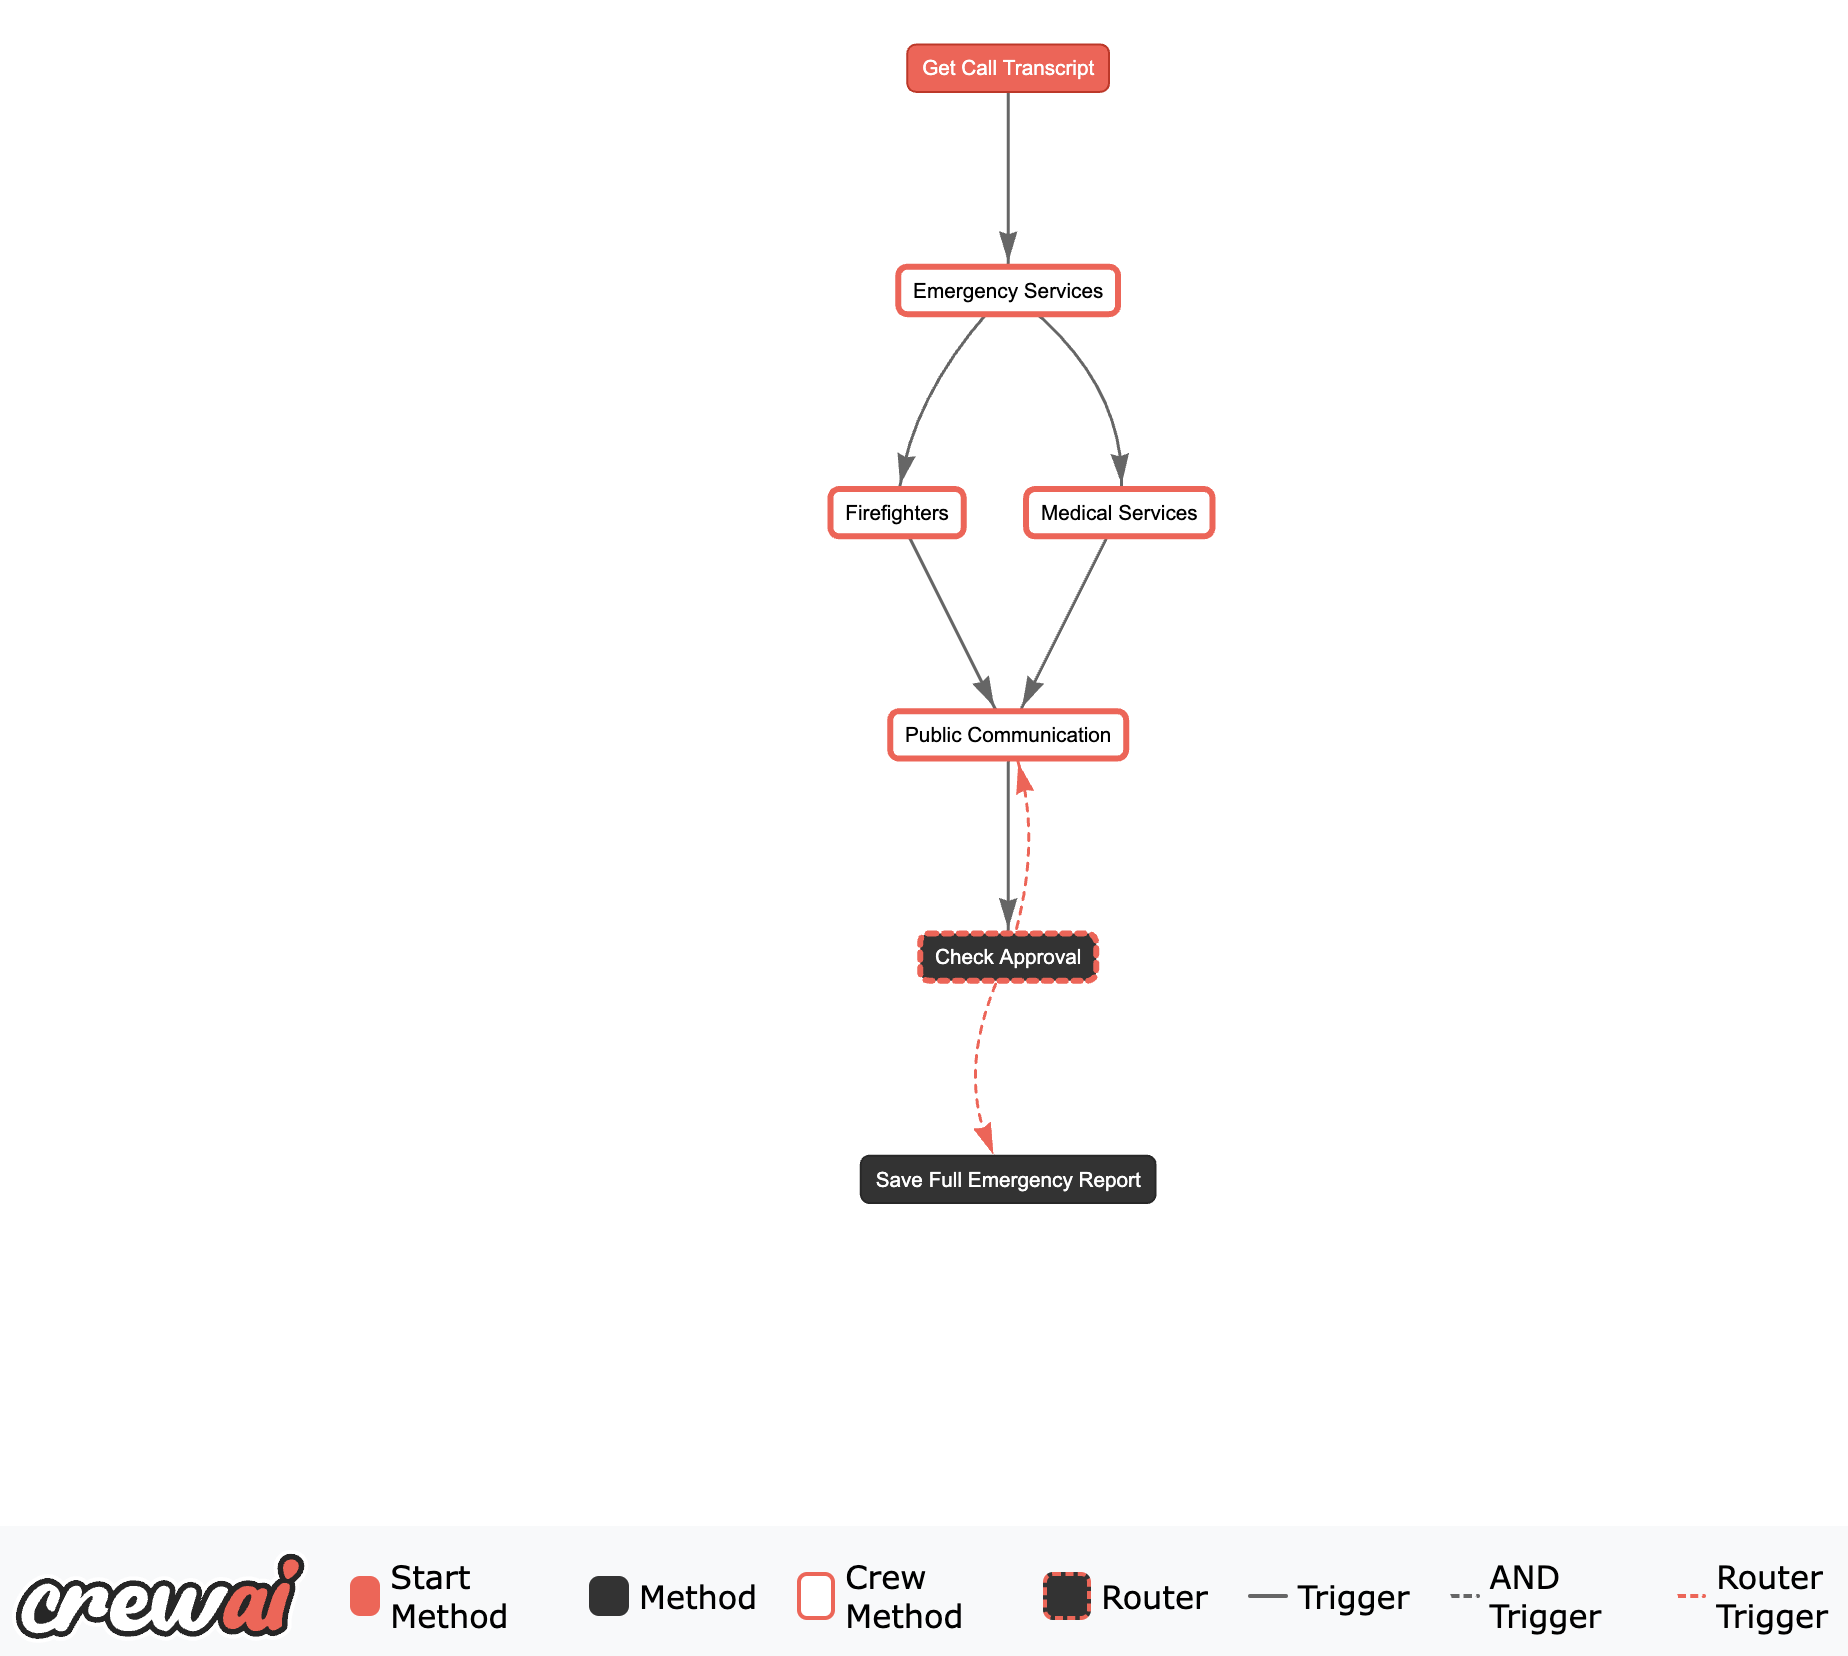
\includegraphics[width=\textwidth]{../figures/coordination_flow.png}
        \end{column}
    \end{columns}
\end{frame}

\subsection{Emergency Planner State}
\begin{frame}[fragile]{Emergency Planner State}
    \begin{lstlisting}[language=Python]
class EmergencyPlannerState:
    call_transcript: str | None
    call_assessment: CallAssessment | None
    firefighters_report: FirefightersReport | None
    medical_report: MedicalReport | None
    public_report: PublicReport | None
    retry_count: int = 0
    \end{lstlisting}
\begin{itemize}
    \item \texttt{call\_transcript}: The transcript of the emergency call
    \item \texttt{call\_assessment}: From \texttt{EmergencyServices} crew
    \item \texttt{firefighters\_response\_report}: From \texttt{Firefighters} crew
    \item \texttt{medical\_response\_report}: From \texttt{MedicalServices} crew
    \item \texttt{public\_communication\_report}: From \texttt{PublicCommunication} crew
    \item \texttt{mayor\_approval\_retry\_count}: Number of mayor approval attempts
\end{itemize}
\end{frame}
